%=====================================================================
%  Physics of Learning  --  Chapter 5
%  The Replica Method II: Spin Glasses, Order Parameters,
%  and the Phases of Learning
%  Style: tufte-handout.   Compile with pdflatex (x2 for refs).
%=====================================================================
\documentclass[nobib,justified]{tufte-handout}

\usepackage{amsmath,amssymb,mathtools}
\usepackage{tikz}
\usetikzlibrary{arrows.meta,positioning,calc}
\usepackage{pgfplots}
\pgfplotsset{compat=1.18}
\usepackage{microtype}

\title{The Replica Method II:\\ Spin Glasses and the Phases of Learning}
\author{Physics of Learning \textbullet\ IIT Madras}
\date{}

\newcommand{\dbar}[1]{\overline{#1}}
\newcommand{\Dz}{\mathcal{D}z}
\newcommand{\Tr}{\operatorname{Tr}}
\definecolor{accent}{HTML}{2A6FA8}
\definecolor{para}{HTML}{B3412B}
\definecolor{retr}{HTML}{2E7D55}
\definecolor{sg}{HTML}{7A5BA6}

\usepackage[most]{tcolorbox}
\newtcolorbox{keyresult}{
  enhanced, colback=accent!6, colframe=accent!75!black,
  boxrule=0.6pt, arc=2pt, left=6pt,right=6pt,top=4pt,bottom=4pt,
  before skip=8pt, after skip=8pt}

\begin{document}
\maketitle
\noindent{\itshape\large Chapter 5}\vspace{4pt}\hrule\vspace{10pt}

\begin{abstract}
\noindent
Chapter~4 developed the replica method on a single spin, where the
$n\to0$ limit was harmless and the overlap was a mere number. Here we
restore the two missing ingredients---a thermodynamic limit and a
\emph{matrix-valued} overlap order parameter---using the
Sherrington--Kirkpatrick (SK) model. We carry the calculation through in
full: the disorder average, the birth of the overlap matrix $q_{ab}$, the
construction of the saddle-point action, the replica-symmetric ansatz, the
explicit $n\to0$ algebra, and the self-consistency equation. We then show
how a phase transition appears as a \emph{bifurcation} of that equation,
locating the spin-glass transition at $T_c=J$. Finally we map the
machinery onto the Hopfield associative memory and read off its phase
diagram, including the storage-capacity singularity at
$\alpha_c\approx0.138$.
\end{abstract}

%---------------------------------------------------------------------
\section{The Sherrington--Kirkpatrick model}

\newthought{Take $N$ spins} $s_i=\pm1$ with all-to-all random couplings:
\begin{keyresult}
\[
  H[\mathbf s] = -\sum_{i<j} J_{ij}\, s_i s_j,
  \qquad J_{ij}\sim\mathcal N\!\Big(0,\frac{J^2}{N}\Big)\ \text{i.i.d.}
\]
\end{keyresult}
\noindent
The $1/N$ scaling of the variance keeps the energy
extensive.\sidenote{Each spin interacts with $N-1$ others; for the total
energy to be $O(N)$ rather than $O(N^2)$, the typical coupling must scale
as $1/\sqrt N$, i.e.\ variance $\propto 1/N$.} The couplings $J_{ij}$ are
the quenched disorder, fixed for a given sample.

\newthought{Why this is the machine-learning prototype.}\label{sec:why}
In a Hopfield network or perceptron, the couplings are built from random
training data $\{\boldsymbol\xi^\mu\}_{\mu=1}^P$---for instance the Hebbian
rule $J_{ij}=\frac1N\sum_\mu \xi_i^\mu\xi_j^\mu$. The quenched disorder
\emph{is the dataset}. The spins are either neuron states (are we in a
memory basin?) or the weights themselves (which configurations fit the
data?). The disorder-averaged free energy therefore computes precisely the
typical-case learning quantities. We treat generic SK first because the
algebra is cleanest, then specialise to Hopfield in
\S\ref{sec:hopfield}.

%---------------------------------------------------------------------
% \section{Disorder average and the birth of the overlap}

% We want $f=-\frac{1}{\beta N}\dbar{\ln Z}$, and apply replicas exactly as
% in Chapter~4:
% \[
%   \dbar{Z^n}
%   = \dbar{\sum_{\{s^a\}}\exp\!\Big(\beta\sum_{a=1}^n\sum_{i<j}
%     J_{ij}\,s_i^a s_j^a\Big)}.
% \]
% The $n$ replicas share the same couplings. Each $J_{ij}$ appears linearly,
% so the disorder average is Gaussian; applying
% $\dbar{e^{Jx}}=e^{\frac12\mathrm{Var}(J)x^2}$ to each pair with
% $x=\beta\sum_a s_i^a s_j^a$ and $\mathrm{Var}=J^2/N$,
% \begin{equation}\label{eq:square}
%   \dbar{Z^n}
%   = \sum_{\{s^a\}}\exp\!\left(\frac{\beta^2 J^2}{2N}
%     \sum_{i<j}\Big(\sum_a s_i^a s_j^a\Big)^2\right).
% \end{equation}
% As before the disorder is gone, leaving a square. Expand it:
% \[
%   \Big(\sum_a s_i^a s_j^a\Big)^2
%   = \sum_{a,b} (s_i^a s_i^b)(s_j^a s_j^b),
% \]
% and extend $\sum_{i<j}\to\frac12\sum_{i,j}$ (the diagonal and double
% counting give $O(1)$ corrections, negligible against the $O(N)$ bulk):
% \[
%   \dbar{Z^n}
%   = \sum_{\{s^a\}}\exp\!\left(\frac{\beta^2 J^2}{4N}
%     \sum_{a,b}\Big(\sum_i s_i^a s_i^b\Big)^2\right).
% \]

% \newthought{The overlap is born.} The object $\sum_i s_i^a s_i^b$ that
% controls everything is, up to $1/N$, the \emph{overlap} between replicas
% $a$ and $b$:
% \begin{keyresult}
% \[
%   q_{ab}\equiv\frac1N\sum_{i=1}^N s_i^a s_i^b .
% \]
% \end{keyresult}
% \noindent
% In Chapter~4 this was the single number $s^a s^b$; now it is an $n\times n$
% matrix, and it is the central object of the whole calculation. In terms of
% it,
% \begin{equation}\label{eq:inq}
%   \dbar{Z^n}
%   = \sum_{\{s^a\}}\exp\!\left(\frac{N\beta^2 J^2}{4}
%     \sum_{a,b} q_{ab}^2\right).
% \end{equation}
% The exponent is now $O(N)$ and depends on the $N$ microscopic spins
% \emph{only through} the macroscopic matrix $q_{ab}$.

% %---------------------------------------------------------------------
% \section{Constructing the saddle-point action}
% \label{sec:action}

% Equation~\eqref{eq:inq} still has $q_{ab}$ \emph{defined} in terms of
% spins. To do the spin sum freely we promote $q_{ab}$ to an independent
% variable, enforcing its definition with a delta function written in
% integral form. For each off-diagonal pair $a<b$ (the diagonal
% $q_{aa}=1$ is fixed):\sidenote{We introduce a conjugate field
% $\hat q_{ab}$, integrated along the imaginary axis. The normalisation
% prefactor contributes only $O(\ln N)$ and is dropped against the $O(N)$
% exponent.}
% \[
%   1 = \int dq_{ab}\,d\hat q_{ab}\;
%       \exp\!\Big(-N\beta^2 J^2\,\hat q_{ab}
%       \big(q_{ab}-\tfrac1N\textstyle\sum_i s_i^a s_i^b\big)\Big).
% \]
% Inserting this for all $a<b$ separates the exponent into a part depending
% only on $\{q,\hat q\}$ and a part containing the spins. Crucially, the
% spin part now \emph{factorises over sites}, because every site $i$ sees
% the same $\hat q$:
% \[
%   \sum_{\{s^a\}}\exp\!\Big(\beta^2 J^2\sum_{a<b}\hat q_{ab}
%      \sum_i s_i^a s_i^b\Big)
%   = \big(\zeta[\hat q]\big)^N,
% \]
% where the \emph{single-site partition function} over the $2^n$ replica
% configurations at one site is
% \[
%   \zeta[\hat q]
%   = \Tr_{\{s^a\}}\exp\!\Big(\beta^2 J^2\sum_{a<b}\hat q_{ab}\,s^a s^b\Big).
% \]
% Collecting everything, $\dbar{Z^n}=\int\!\prod_{a<b}dq_{ab}\,d\hat q_{ab}\,
% e^{N\Phi[q,\hat q]}$ with the action
% \begin{keyresult}
% \[
%   \Phi[q,\hat q]
%   = \frac{\beta^2 J^2}{4}\sum_{a,b} q_{ab}^2
%   - \beta^2 J^2\sum_{a<b}\hat q_{ab}\,q_{ab}
%   + \ln\zeta[\hat q].
% \]
% \end{keyresult}
% \noindent
% Three pieces: the bare $q^2$ energy, the Legendre coupling between $q$ and
% its conjugate, and the single-site term $\ln\zeta$.

%---------------------------------------------------------------------
%---------------------------------------------------------------------
\section{Disorder average and the birth of the overlap}

We want $f=-\frac{1}{\beta N}\dbar{\ln Z}$, and apply replicas exactly as
in Chapter~4:
\[
  \dbar{Z^n}
  = \dbar{\sum_{\{s^a\}}\exp\!\Big(\beta\sum_{a=1}^n\sum_{i<j}
    J_{ij}\,s_i^a s_j^a\Big)}.
\]
The $n$ replicas share the same couplings. Each $J_{ij}$ appears linearly,
so the disorder average is Gaussian; applying
$\dbar{e^{Jx}}=e^{\frac12\mathrm{Var}(J)x^2}$ to each pair with
$x=\beta\sum_a s_i^a s_j^a$ and $\mathrm{Var}=J^2/N$,
\begin{equation}\label{eq:square}
  \dbar{Z^n}
  = \sum_{\{s^a\}}\exp\!\left(\frac{\beta^2 J^2}{2N}
    \sum_{i<j}\Big(\sum_a s_i^a s_j^a\Big)^2\right).
\end{equation}
As before the disorder is gone, leaving a square. Expand it:
\[
  \Big(\sum_a s_i^a s_j^a\Big)^2
  = \sum_{a,b} (s_i^a s_i^b)(s_j^a s_j^b),
\]
and extend $\sum_{i<j}\to\frac12\sum_{i,j}$ (the diagonal and double
counting give $O(1)$ corrections, negligible against the $O(N)$ bulk):
\begin{equation}\label{eq:beforeq}
  \dbar{Z^n}
  = \sum_{\{s^a\}}\exp\!\left(\frac{\beta^2 J^2}{4N}
    \sum_{a,b}\Big(\sum_i s_i^a s_i^b\Big)^2\right).
\end{equation}

\newthought{The overlap is born.} The object $\sum_i s_i^a s_i^b$ that
controls everything is, up to $1/N$, the \emph{overlap} between replicas
$a$ and $b$:
\begin{keyresult}
\[
  q_{ab}\equiv\frac1N\sum_{i=1}^N s_i^a s_i^b .
\]
\end{keyresult}
\noindent
In Chapter~4 this was the single number $s^a s^b$; now it is an $n\times n$
matrix, and it is the central object of the whole calculation. In terms of
it,
\begin{equation}\label{eq:inq}
  \dbar{Z^n}
  = \sum_{\{s^a\}}\exp\!\left(\frac{N\beta^2 J^2}{4}
    \sum_{a,b} q_{ab}^2\right).
\end{equation}
The exponent is now $O(N)$ and depends on the $N$ microscopic spins
\emph{only through} the macroscopic matrix $q_{ab}$.

%---------------------------------------------------------------------
\section{Decoupling the spins: the delta-function trick}
\label{sec:delta}

Equation~\eqref{eq:inq} cannot yet be summed over the spins, because the
exponent contains $q_{ab}^2=\big(\frac1N\sum_i s_i^a s_i^b\big)^2$, which
couples \emph{every site $i$ to every site $j$} through the square. The
strategy is to introduce $q_{ab}$ as a new \emph{independent} integration
variable, so that the exponent becomes linear in the spins and the site
sum factorises. The price is one constraint per replica pair, enforced by a
Dirac delta.

\newthought{A single scalar first.} Forget replicas for a moment and
consider one macroscopic variable $Q=\frac1N\sum_i \phi_i$, where $\phi_i$
are some microscopic quantities. To trade the microscopic $\phi_i$ for the
macroscopic $Q$, insert the identity\sidenote{This is just
$1=\int dQ\,\delta\!\big(Q-\frac1N\sum_i\phi_i\big)$: the delta forces $Q$
to equal the empirical mean. The factor of $N$ inside, $\delta(NQ-\dots)$
versus $\delta(Q-\dots)$, only rescales the (irrelevant) normalisation.}
\begin{equation}\label{eq:scalardelta}
  1 = \int dQ\;\delta\!\Big(NQ-\sum_i\phi_i\Big).
\end{equation}
Now write the delta in its \emph{Fourier (integral) representation},
\begin{equation}\label{eq:fourier}
  \delta(x)=\int_{-i\infty}^{+i\infty}\frac{d\hat Q}{2\pi i}\;
            e^{-\hat Q\,x},
\end{equation}
where $\hat Q$ is a conjugate variable integrated along the imaginary
axis.\sidenote{Equivalently $\delta(x)=\int\frac{dk}{2\pi}e^{-ikx}$ with
$\hat Q=ik$. The imaginary-axis contour is what makes the later
saddle-point well defined. We absorb constant prefactors like $2\pi i$ into
the measure and stop writing them, since they contribute only $O(\ln N)$
to an $O(N)$ exponent.} Substituting \eqref{eq:fourier} into
\eqref{eq:scalardelta} with $x=NQ-\sum_i\phi_i$ gives
\begin{equation}\label{eq:scalarfull}
  1 = \int dQ\,d\hat Q\;
      \exp\!\Big(-\hat Q\big(NQ-\textstyle\sum_i\phi_i\big)\Big)
    = \int dQ\,d\hat Q\;
      \exp\!\Big(-N\hat Q\,Q + \hat Q\textstyle\sum_i\phi_i\Big).
\end{equation}
The crucial feature: in the last form the microscopic variables $\phi_i$
now appear \emph{linearly}, inside $\hat Q\sum_i\phi_i=\sum_i\hat Q\phi_i$
--- a sum of independent single-site terms. The coupling has been moved
into the new pair $(Q,\hat Q)$.

\newthought{Now the matrix version.} We apply exactly this device to each
replica pair. Here $\phi_i\to s_i^a s_i^b$ and $Q\to q_{ab}$, with a
separate conjugate $\hat q_{ab}$ for every pair $a<b$ (the diagonal
$q_{aa}=1$ is fixed, since $(s_i^a)^2=1$, and needs no constraint). For each
$a<b$ insert
\begin{equation}\label{eq:matdelta}
  1 = \int dq_{ab}\,d\hat q_{ab}\;
      \exp\!\Big(-N\,\tilde q_{ab}\,q_{ab}
      + \tilde q_{ab}\textstyle\sum_i s_i^a s_i^b\Big),
\end{equation}
where I temporarily call the conjugate $\tilde q_{ab}$. It is convenient to
rescale it as $\tilde q_{ab}=\beta^2 J^2\,\hat q_{ab}$ so that later
formulas are clean; this is just a change of integration variable. With
that rescaling,
\begin{equation}\label{eq:matdelta2}
  1 = \int dq_{ab}\,d\hat q_{ab}\;
      \exp\!\Big(-N\beta^2 J^2\,\hat q_{ab}\,q_{ab}
      + \beta^2 J^2\,\hat q_{ab}\textstyle\sum_i s_i^a s_i^b\Big).
\end{equation}

\newthought{Insert into $\dbar{Z^n}$.} Multiply
Eq.~\eqref{eq:inq} by one factor of \eqref{eq:matdelta2} for each pair
$a<b$. The exponent now splits into three groups of terms:
\begin{equation}\label{eq:split}
  \dbar{Z^n}
  = \int\!\prod_{a<b}dq_{ab}\,d\hat q_{ab}\;
    \exp\!\Big(
      \underbrace{\tfrac{N\beta^2 J^2}{4}\textstyle\sum_{a,b}q_{ab}^2}_{\text{(i) from \eqref{eq:inq}}}
      \;-\;
      \underbrace{N\beta^2 J^2\textstyle\sum_{a<b}\hat q_{ab}q_{ab}}_{\text{(ii) constraint, $q$-part}}
    \Big)\;
    \underbrace{\sum_{\{s^a\}}\exp\!\Big(\beta^2 J^2\textstyle\sum_{a<b}\hat q_{ab}\sum_i s_i^a s_i^b\Big)}_{\text{(iii) constraint, spin-part}} .
\end{equation}
Term (i) replaced the empirical $q_{ab}$ by the independent variable, which
is legitimate \emph{because} the delta enforces their equality. Terms (i)
and (ii) depend only on $\{q,\hat q\}$ and pull out of the spin sum. All the
spin dependence is now in (iii), and---this is the payoff---it is
\emph{linear} in the bilinears $s_i^a s_i^b$.

\newthought{Why the spin part factorises over sites.} Look at the exponent
of (iii) and exchange the order of summation, pulling the site sum
outward:
\[
  \beta^2 J^2\sum_{a<b}\hat q_{ab}\sum_i s_i^a s_i^b
  \;=\;
  \sum_{i=1}^N \underbrace{\Big(\beta^2 J^2\sum_{a<b}\hat q_{ab}\,s_i^a s_i^b\Big)}_{\text{depends on site $i$ only}} .
\]
The total exponent is a \emph{sum over sites} of a term involving only the
$n$ replica-spins at that one site. The exponential of a sum is a product
of exponentials, and the spin sum $\sum_{\{s^a\}}=\prod_i\sum_{\{s_i^a\}}$
also factorises over sites, so
\[
  \sum_{\{s^a\}}\exp\!\Big(\sum_i \beta^2 J^2\!\sum_{a<b}\hat q_{ab}s_i^a s_i^b\Big)
  =\prod_{i=1}^N\;\sum_{\{s_i^a\}}\exp\!\Big(\beta^2 J^2\!\sum_{a<b}\hat q_{ab}s_i^a s_i^b\Big).
\]
Every factor in the product is \emph{identical}---the site label $i$ is a
dummy, since each site sees the same $\hat q_{ab}$. Calling the common
single-site sum
\begin{equation}\label{eq:zeta}
  \zeta[\hat q]
  = \Tr_{\{s^a\}}\exp\!\Big(\beta^2 J^2\sum_{a<b}\hat q_{ab}\,s^a s^b\Big),
  \qquad \Tr_{\{s^a\}}\equiv\!\!\sum_{s^1=\pm1}\!\!\cdots\!\!\sum_{s^n=\pm1},
\end{equation}
the product is simply $\zeta[\hat q]^N$. (Here $s^a$ denotes the $n$ replica
spins \emph{at one site}; the $2^n$ terms of the trace are all the
configurations of those $n$ spins.)

\newthought{The action.} Writing $\zeta^N=e^{N\ln\zeta}$ and collecting
(i), (ii), (iii), we obtain $\dbar{Z^n}=\int\!\prod_{a<b}dq_{ab}\,
d\hat q_{ab}\,e^{N\Phi[q,\hat q]}$ with
\begin{keyresult}
\[
  \Phi[q,\hat q]
  = \frac{\beta^2 J^2}{4}\sum_{a,b} q_{ab}^2
  - \beta^2 J^2\sum_{a<b}\hat q_{ab}\,q_{ab}
  + \ln\zeta[\hat q].
\]
\end{keyresult}
\noindent
Three pieces: the bare $q^2$ energy (i), the Legendre coupling between $q$
and its conjugate (ii), and the single-site term $\ln\zeta$ (iii). Every
term is $O(N)$ in the exponent, which is what makes the saddle-point
evaluation of the next section exact as $N\to\infty$.

\section{The saddle point}

Because every term in the exponent is $O(N)$, the integral is dominated as
$N\to\infty$ by its saddle point (Laplace's method): $\dbar{Z^n}\approx
e^{N\Phi[q^\star,\hat q^\star]}$, with $\Phi$ extremised. \emph{This is the
qualitative break from Chapter~4}: there was no $N$ there, hence no saddle;
here the saddle is the physics.

\newthought{Extremise over $q_{ab}$} (off-diagonal):
\[
  \frac{\partial\Phi}{\partial q_{ab}}=0
  \;\Rightarrow\;
  \beta^2 J^2 q_{ab}-\beta^2 J^2\hat q_{ab}=0
  \;\Rightarrow\; \hat q_{ab}=q_{ab}.
\]
The conjugate field simply equals the overlap at the saddle.

\newthought{Extremise over $\hat q_{ab}$:}
\[
  \frac{\partial\Phi}{\partial\hat q_{ab}}=0
  \;\Rightarrow\;
  q_{ab}=\frac{1}{\zeta}\Tr\Big[s^a s^b\,
     e^{\beta^2 J^2\sum_{c<d}\hat q_{cd}s^c s^d}\Big]
  =\langle s^a s^b\rangle_{\text{eff}}.
\]
This is the \emph{self-consistency equation}: the overlap equals the
thermal average of $s^a s^b$ in an effective single-site problem whose
couplings are the overlaps themselves. The loop is closed---but to solve
it, and to take $n\to0$, we must assume a structure for the matrix.

%---------------------------------------------------------------------
\section{The replica-symmetric ansatz}
\label{sec:rs}

\newthought{The simplest guess} is that all replicas are equivalent
(\emph{replica symmetry}, RS):
\[
  q_{ab}=q\ (a\neq b),\qquad q_{aa}=1,\qquad \hat q_{ab}=q\ (a\neq b).
\]
We now evaluate each piece of $\Phi$ as an explicit function of $n$ and
$q$.

\newthought{Piece 1 --- the $q^2$ term.} The sum $\sum_{a,b}q_{ab}^2$ runs
over all $n^2$ entries: $n$ diagonal entries equal to $1$, and $n(n-1)$
off-diagonal entries equal to $q^2$. Thus
\[
  \frac{\beta^2 J^2}{4}\sum_{a,b}q_{ab}^2
  = \frac{\beta^2 J^2}{4}\big[n + n(n-1)q^2\big].
\]

\newthought{Piece 2 --- the coupling term.} The sum over $a<b$ has
$\binom n2=\frac{n(n-1)}{2}$ pairs, each contributing
$\hat q_{ab}q_{ab}=q^2$:
\[
  -\beta^2 J^2\sum_{a<b}\hat q_{ab}q_{ab}
  = -\beta^2 J^2\,\frac{n(n-1)}{2}\,q^2 .
\]

\newthought{Piece 3 --- the single-site trace.} We must evaluate
\[
  \zeta = \Tr\exp\!\Big(\beta^2 J^2 q\sum_{a<b}s^a s^b\Big).
\]
Use $\sum_{a<b}s^a s^b=\tfrac12\big[(\sum_a s^a)^2-n\big]$ (since
$(s^a)^2=1$):
\[
  \zeta = e^{-\beta^2 J^2 q\,n/2}\,
    \Tr\exp\!\Big(\tfrac{\beta^2 J^2 q}{2}\big(\textstyle\sum_a s^a\big)^2\Big).
\]
The square couples replicas; \emph{Hubbard--Stratonovich} decouples them,
exactly as in Chapter~4:\sidenote{$e^{\frac12 a m^2}=\int\Dz\,
e^{\sqrt a\,z m}$ with $a=\beta^2 J^2 q$, so $\sqrt a=\beta J\sqrt q$.}
\[
  \zeta = e^{-\beta^2 J^2 q\,n/2}
    \int\Dz\,\Big[\Tr_{s}\,e^{\beta J\sqrt q\,z\,s}\Big]^n
  = e^{-\beta^2 J^2 q\,n/2}
    \int\Dz\,\big[2\cosh(\beta J\sqrt q\,z)\big]^n.
\]
\emph{The same integral structure as the toy model}, but now the effective
field strength $\beta J\sqrt q$ is self-generated by the overlap rather
than externally fixed.

%---------------------------------------------------------------------
\section{Taking $n\to0$ explicitly}
\label{sec:nto0}

We need $f=-\frac1\beta\lim_{n\to0}\frac1n\Phi$. Take each piece divided by
$n$, using $n(n-1)/n=n-1\to-1$.

\newthought{The polynomial pieces:}
\begin{align*}
  \frac1n\Big[\tfrac{\beta^2 J^2}{4}\big(n+n(n-1)q^2\big)
     -\tfrac{\beta^2 J^2}{2}n(n-1)q^2\Big]
  &\xrightarrow{n\to0}
  \tfrac{\beta^2 J^2}{4}(1-q^2)+\tfrac{\beta^2 J^2}{2}q^2 \\
  &= \tfrac{\beta^2 J^2}{4}\big(1+q^2\big).
\end{align*}

\newthought{The $\ln\zeta$ piece.} Write
$\zeta=e^{-\beta^2 J^2 q\,n/2}I_n$ with
$I_n=\int\Dz\,[2\cosh(\beta J\sqrt q\,z)]^n$. Since $I_0=\int\Dz=1$, we
have $\ln I_n=n\,\partial_n I_n|_{0}+O(n^2)$ with
$\partial_n[2\cosh]^n|_0=\ln(2\cosh)$. Hence
\[
  \frac1n\ln\zeta\xrightarrow{n\to0}
  -\frac{\beta^2 J^2 q}{2}
  +\int\Dz\,\ln\!\big[2\cosh(\beta J\sqrt q\,z)\big].
\]

\newthought{Collecting} (and using
$\tfrac{\beta^2J^2}{4}(1+q^2)-\tfrac{\beta^2J^2}{2}q
=\tfrac{\beta^2J^2}{4}(1-q)^2$), the replica-symmetric free energy is
\begin{keyresult}
\[
  -\beta f
  = \frac{\beta^2 J^2}{4}(1-q)^2
  + \int\Dz\,\ln\!\big[2\cosh(\beta J\sqrt q\,z)\big].
\]
\end{keyresult}
\noindent
\textbf{Consistency check.} Formally setting $q=0$ collapses this to
$\frac{\beta^2 J^2}{4}+\ln 2$---the Chapter~4 answer with $\sigma\to J$.
The toy model was the $q=0$ slice of the spin glass.

%---------------------------------------------------------------------
\section{The order-parameter equation}

Extremise the free energy over $q$. Differentiating the integral and
integrating by parts in $z$\sidenote{Using
$\frac{d}{dq}\ln 2\cosh(\beta J\sqrt q z)
=\tanh(\beta J\sqrt q z)\cdot\frac{\beta J z}{2\sqrt q}$, then
$\int\Dz\,z\,g(z)=\int\Dz\,g'(z)$ (Gaussian integration by parts), and
$\frac{d}{dz}\tanh=\beta J\sqrt q\,\mathrm{sech}^2$. The
$\frac{\beta^2J^2}{2}$ terms cancel, leaving the result.} gives the clean
fixed-point equation
\begin{keyresult}
\[
  q = \int\Dz\,\tanh^2\!\big(\beta J\sqrt q\,z\big).
\]
\end{keyresult}
\noindent
Compare the toy-model magnetisation
$\dbar{\langle s\rangle^2}=\dbar{\tanh^2(\beta h)}$: identical in form, but
now $q$ appears on \emph{both} sides. The overlap is self-generated---each
spin feels an effective random field $\beta J\sqrt q\,z$ created
collectively by all the others through $q$ itself.\sidenote{This is the
\emph{cavity-field} picture: remove one spin, and the field it would feel
is a Gaussian of variance $J^2 q$ produced by the rest of the system.}

%---------------------------------------------------------------------
\section{Where the singularity is: the spin-glass transition}
\label{sec:transition}

\marginnote{%
\centering
\begin{tikzpicture}
\begin{axis}[
  width=4.7cm,height=3.7cm,
  xlabel={\footnotesize $T/J$}, ylabel={\footnotesize $q$},
  xmin=0,xmax=2,ymin=0,ymax=1.05,
  xtick={1}, xticklabels={$T_c$}, ytick={0,1},
  axis lines=left, every axis plot/.append style={line width=1pt},
  ylabel style={rotate=-90}]
  % q grows from 0 below Tc; schematic q ~ (1-T) for T<1
  \addplot[sg,domain=0:1,samples=60]{(1-x)^1.0};
  \addplot[para,domain=1:2,samples=2]{0};
  \draw[gray,dashed] (axis cs:1,0)--(axis cs:1,1.05);
\end{axis}
\end{tikzpicture}\\[2pt]
\footnotesize The order parameter $q$ bifurcates from zero at $T_c=J$.
For $T>T_c$: paramagnet ($q=0$). For $T<T_c$: spin glass ($q>0$).}

We now locate the non-analyticity. Set $J=1$ and study the fixed-point
equation as $\beta=1/T$ varies.

\newthought{$q=0$ is always a solution} (the paramagnet): if $q=0$ the
$\tanh$ argument vanishes and $\tanh^2(0)=0$, consistent. The transition is
the point where a \emph{nonzero} branch splits off.

\newthought{Expand for small $q$.} For small argument
$\tanh^2(x)\approx x^2=\beta^2 q z^2$, so
\[
  q=\int\Dz\,\beta^2 q\,z^2
   =\beta^2 q\underbrace{\int\Dz\,z^2}_{=1}
   =\beta^2 q .
\]
Thus $q(1-\beta^2)=0$: a nonzero solution becomes possible exactly when
the coefficient reaches unity,
\begin{keyresult}
\[
  \beta_c^2=1 \quad\Longrightarrow\quad T_c=J .
\]
\end{keyresult}
\noindent
\textbf{This is the singularity.} For $T>T_c$ only $q=0$ exists
(paramagnetic phase: disordered, no frozen structure). For $T<T_c$ a stable
$q>0$ branch appears (spin-glass phase: spins freeze into a random but
rigid pattern). The free energy $f(T)$ is analytic on each side but has a
non-analytic kink at $T_c$---its second derivative is discontinuous. That
discontinuity \emph{is} the phase transition, and it arose purely from the
bifurcation of the saddle-point equation.

\newthought{The general mechanism.} A phase transition appears in this
formalism wherever the \emph{number or stability of solutions} to the
saddle-point equation changes. A new branch appearing (or an existing one
vanishing) is a singularity of $\dbar{\ln Z}$. This is the precise content
of the slogan ``non-analyticities of the free energy are phase
transitions.''

%---------------------------------------------------------------------
\section{A caveat: when replica symmetry fails}

The RS ansatz is not always correct. Computing the entropy from the RS free
energy, one finds it goes \emph{negative} at low temperature---impossible
for a discrete spin system.\sidenote{This is the de~Almeida--Thouless
instability: below a line in the $(T,h)$ plane the RS saddle is no longer a
maximum in replica space. The cure is Parisi's \emph{replica symmetry
breaking}, in which $q_{ab}$ is not uniform but hierarchically structured,
described by a function $q(x)$, $x\in[0,1]$, and the order parameter
becomes a whole distribution of overlaps $P(q)$.} The implication for the
$n\to0$ trick is sharp: the continuation is \emph{not} innocent. The
structure one assumes for the matrix as $n\to0$ determines the answer, and
the correct structure (RS, or one of the RSB schemes) is a nontrivial
property of the problem. The full Parisi treatment is beyond these notes;
what matters here is that the \emph{location of a transition}---a bifurcation
of the order-parameter equation---is already visible at RS level.

%---------------------------------------------------------------------
\section{The phases of learning: Hopfield memory}
\label{sec:hopfield}

\newthought{Now make the disorder data.} Store $P=\alpha N$ random patterns
$\{\boldsymbol\xi^\mu\}$, $\xi_i^\mu=\pm1$, via the Hebbian couplings
\[
  J_{ij}=\frac1N\sum_{\mu=1}^P \xi_i^\mu\xi_j^\mu .
\]
The quenched disorder is now the stored dataset. The replica calculation
proceeds as above, but with \emph{two} kinds of order parameter:
\begin{itemize}
\item the \emph{retrieval overlap} $m=\frac1N\sum_i \langle s_i\rangle
  \xi_i^1$ with the pattern we are trying to recall;
\item the \emph{spin-glass overlap} $q=\frac1N\sum_i\langle s_i\rangle^2$
  generated by the other $P-1$ patterns acting as quenched noise.
\end{itemize}
The interference from the non-retrieved patterns plays exactly the role of
the random field in the toy model---a self-consistent Gaussian noise of
variance set by $\alpha$ and $q$.

\newthought{The phase diagram} in the $(\alpha,T)$ plane has three regions,
each a different solution branch of the saddle-point equations.
\marginnote{%
\centering
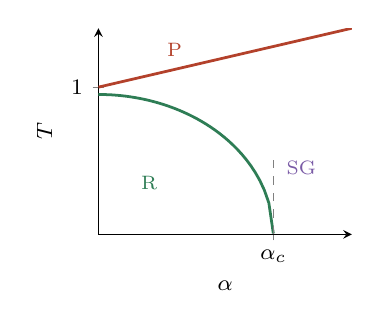
\begin{tikzpicture}
\begin{axis}[
  width=4.8cm,height=4.2cm,
  xlabel={\footnotesize $\alpha$}, ylabel={\footnotesize $T$},
  xmin=0,xmax=0.2,ymin=0,ymax=1.4,
  xtick={0.138}, xticklabels={\footnotesize $\alpha_c$},
  ytick={1}, yticklabels={\footnotesize $1$},
  axis lines=left]
  % paramagnetic boundary T=1+sqrt(alpha) approx (schematic)
  \addplot[para,line width=1pt,domain=0:0.2,samples=40]{1+2.0*x};
  % retrieval region boundary (schematic curve down to alpha_c)
  \addplot[retr,line width=1pt,domain=0:0.138,samples=40]
    {0.95*(1-(x/0.138)^2)^0.5};
  \node[para,font=\scriptsize] at (axis cs:0.06,1.25){P};
  \node[retr,font=\scriptsize] at (axis cs:0.04,0.35){R};
  \node[sg,font=\scriptsize] at (axis cs:0.16,0.45){SG};
  \draw[gray,dashed](axis cs:0.138,0)--(axis cs:0.138,0.55);
\end{axis}
\end{tikzpicture}\\[2pt]
\footnotesize Hopfield phases: \textcolor{para}{P}aramagnetic,
\textcolor{retr}{R}etrieval, \textcolor{sg}{S}pin-\textcolor{sg}{G}lass.
Retrieval ends at $\alpha_c\approx0.138$.}
\begin{description}
\item[Retrieval (R)] --- low $\alpha$, low $T$: a solution with $m\approx1$
  exists; the network recalls the stored memory. The free energy has a
  minimum at large overlap with a pattern.
\item[Spin glass (SG)] --- high $\alpha$: only $m=0,\,q>0$ solutions
  survive; the network freezes into spurious mixtures and memories are
  destroyed.
\item[Paramagnet (P)] --- high $T$: $m=q=0$; thermal noise melts all
  structure.
\end{description}

\newthought{The capacity singularity.} The retrieval/spin-glass boundary at
low temperature sits at the storage capacity
\begin{keyresult}
\[
  \alpha_c \approx 0.138 .
\]
\end{keyresult}
\noindent
This number is precisely the value of $\alpha$ at which the $m\neq0$
retrieval branch of the saddle-point equations \emph{ceases to exist}---the
same bifurcation mechanism as the SK transition in \S\ref{sec:transition},
now in the data-load parameter $\alpha$ rather than temperature. Beyond
$\alpha_c$ the memory is overloaded: adding more patterns destroys the
ability to recall any of them. The crossover that was perfectly smooth for
one neuron in Chapter~4 has become a sharp, computable threshold.

%---------------------------------------------------------------------
\section{The throughline}

The single spin of Chapter~4 taught the \emph{mechanism}: average the log
via replicas; the shared disorder couples them; an overlap is born. This
chapter added the two ingredients that make the method powerful and
genuinely hard:
\begin{enumerate}
\item a \emph{thermodynamic limit}, turning the calculation into a saddle
  point over the overlap;
\item a \emph{matrix order parameter} $q_{ab}$, whose $n\to0$
  structure---replica-symmetric or broken---encodes the real physics.
\end{enumerate}
And the payoff is concrete: a phase transition is a bifurcation of the
order-parameter equation, and quantities such as the Hopfield capacity
$\alpha_c\approx0.138$ are read directly off where a solution branch of
$\dbar{\ln Z}$ appears or vanishes. The free energy is, in the end, the
generating function for everything a learning system typically does.

\end{document}
